
\subsection*{Què és la tecnologia Li-Fi i com funciona?}
\addcontentsline{toc}{subsection}{Què és la tecnologia Li-Fi i com funciona?}

Li-Fi (Light Fidelity) és una forma de comunicació sense fil que utilitza llum LED (diodos emissors de llum) per a transmetre dades a una velocitat molt alta. Aquesta tecnologia funciona modulant la intensitat de la llum a una taxa molt ràpida, invisible per a l'ull humà, per transmetre informació.

La tecnologia Li-Fi suposa una gran millora en comparació amb el Wi-Fi a tots els nivells. Per començar, la velocitat de transmissió és fins a 100 vegades més ràpida!

\begin{figure}[h!]
    \centering
    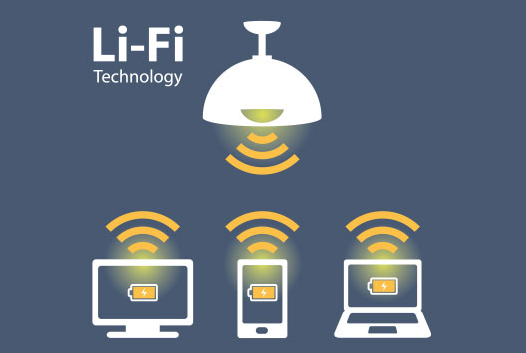
\includegraphics[width=80mm]{lifi.png}
    \caption{Tecnologia Li-Fi}
\end{figure}


\subsection*{Avantatges de Li-Fi}
\addcontentsline{toc}{subsection}{Avantatges de Li-Fi}

\subsubsection*{Sostenibilitat: menor cost i més eficiència}

Els seus avantatges no estan només a la velocitat. S'estima que en un futur proper podrem transmetre dades a través de l'energia solar, cosa que facilitarà l'accés a persones sense Internet i amb recursos d'electricitat limitats. El funcionament de la tecnologia Li-Fi estalviarà costos a les llars i, sobretot, als llocs de treball. Podria funcionar sense dispositius electrònics com ara rúters, mòdems, repetidors, amplificadors d'ona i antenes.

Aquests dispositius, que actualment estan connectats a la xarxa elèctrica les 24 hores del dia, els 7 dies de la setmana, deixarien de consumir electricitat i la seva funció seria reemplaçada per una bombeta LED, que en la majoria dels casos ja està encesa durant el horari de treball, per tant, no significaria un cost extra.

La principal diferència entre Li-Fi i altres formes de comunicació òptica, com ara la fibra òptica, és que Li-Fi no utilitza fils físics per a la transmissió de dades. En canvi, transmet les dades mitjançant la il·luminació LED ja existent en un entorn. Aquesta tecnologia pot oferir velocitats de transmissió de dades molt altes i també pot ser utilitzada en entorns on les comunicacions per ones de ràdio poden ser limitades, com ara en hospitals o en aules on l'ús de ones de ràdio pot estar restringit.

\subsubsection*{Seguretat contra atacs}

Com que cal estar en contacte directe amb l'emissor de feix de llum LED, es reforça la seguretat
informàtica. Només els dispositius il·luminats per la mateixa bombeta poden interconnectar-se entre si,
eliminant atacs o intents d'entrada no autoritzats des de dispositius fora del nostre espectre de
llum.
Una soluci´o brillant, més segura, més ràpida i eficient per optimitzar la nostra connexió amb el
món.


\subsection*{Incovenients de Li-Fi}
\addcontentsline{toc}{subsection}{Incovenients de Li-Fi}

Encara que la tecnologia Li-Fi ofereix algunes avantatges, també té alguns inconvenients i limitacions que poden afectar la seva adopció i implementació:


\begin{itemize}
    \item Dependència de la llum visible: La transmissió de dades a través de Li-Fi depèn de la llum visible, de manera que la comunicació pot veure afectada per la falta de llum, com en entorns foscos o quan les llums estan apagades.
    \item Limitacions d'abast: La cobertura de Li-Fi és generalment més limitada que la del Wi-Fi, ja que la llum no penetra a través de parets o altres obstacles com ho fa la radiació de radiofreqüència.
    \item Interferència de la llum solar: La llum solar pot interferir amb la transmissió de dades Li-Fi, ja que les dues fonts de llum poden ser captades pel receptor, provocant interferències i afectant el rendiment de la comunicació.
    \item Limitacions de mobilitat: La tecnologia Li-Fi pot ser menys adequada per a dispositius en moviment, ja que requereix una connexió visual constant amb la font de llum per a una transmissió de dades eficaç.
\end{itemize}








\subsection*{Wi-Fi vs Li-Fi}
\addcontentsline{toc}{subsection}{Wi-Fi vs Li-Fi}


\begin{table}[h]
\centering
\begin{tabular}{ | p{5.5em} | p{19em} | p{19em} | } 
\hline
 & Wi-Fi  (Wireless Fidelity)& Li-Fi  (Light Fidelity)\\
\hline
Avantatges & més interferència, no atraviesa l'aigua de mar, funciona en regions menys denses 
& menys interferència, pot atravesar l'aigua de mar, funciona en regions denses \\
\hline
Aplicació & S'utilitza per navegar per Internet amb l'ajuda de punts d'accés Wi-Fi 
& S'utilitza en aerolínies, exploracions submarines, quiròfans a hospitals, oficines i locals domèstics per a la transferència de dades i la navegació per Internet \\
\hline
Distancia de cobertura & uns 32 metres, varia segons la potència de transmissió i el tipus d'antena
& uns 10 metres \\
\hline
Densitat de dades & Funciona en entorns menys densos a causa de problemes relacionats amb la interferència 
& Funciona en entorns de alta densitat \\
\hline
Interferències & Diverses fonts d'interferències de ràdio poden interrompre el funcionament d'una xarxa Wi-Fi 
& No tenen problemes de interferència similar a les ones de radiofreqüència\\
\hline
Operació & Wi-Fi transmet dades utilitzant ones de radio amb l'ajuda d'un encaminador Wi-Fi
& LiFi transmet dades utilitzant fonts de llum (actualment focus LED) \\
\hline
Privacitat &  Wi-Fi és menys segur perquè el senyal no pot ser bloquejat per parets i la majoria dels objectes 
& Amb LiFi, les parets bloquegen la llum, i per tant, proporcionarà una transferència de dades més segura \\
\hline
\end{tabular}
\end{table}




\subsection*{Productes Li-Fi}
\addcontentsline{toc}{subsection}{Productes Li-Fi}

\subsubsection*{LiFiMAX Compact}

El LiFiMAX Compact és un sistema plug-and-play revolucionari que ofereix una connexió a Internet sense fils increïblement ràpida, segura i fiable a través de la llum invisible.


\begin{figure}[h!]
    \centering
    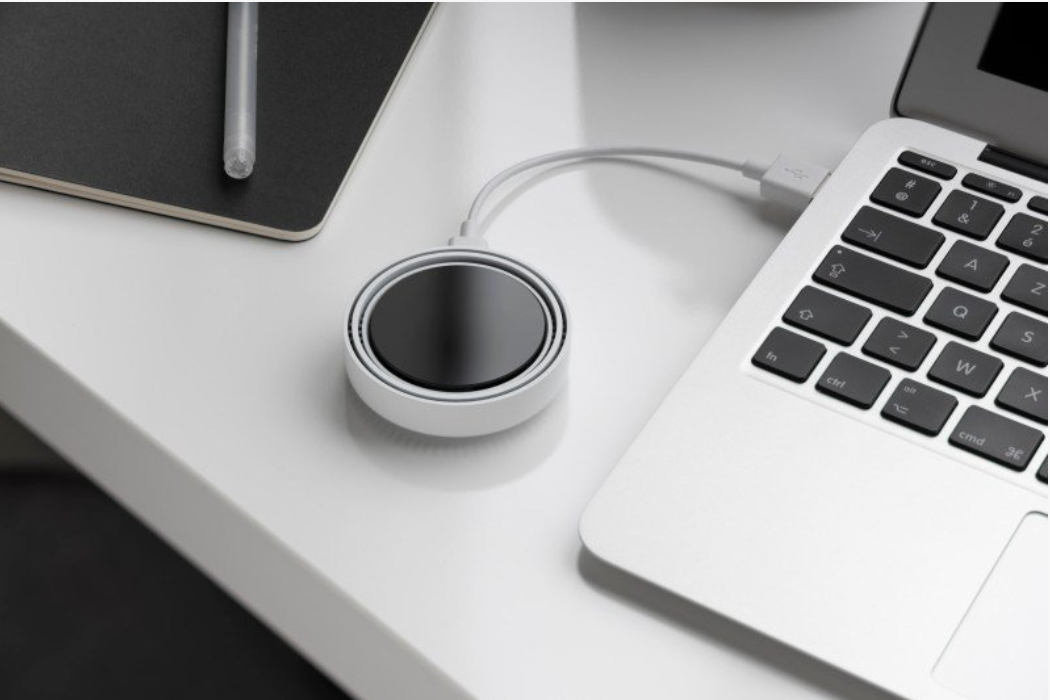
\includegraphics[width=80mm]{lifimaxaa.png}
    \caption{Li-Fi MAX}
\end{figure}

\subsubsection*{LiFiMAX Tab}

LiFiMAX Tab és una tauleta que es connecta a Internet mitjançant llum invisible. Aquesta tauleta és una alternativa revolucionària als dispositius actuals amb Wi-Fi. LiFiMAX Tab permet als usuaris connectar-se a través d'una connexió estable, ràpida i sense radiofreqüències que pot ser difícil d'interceptar fora de l'habitació. És perfecte per a l'ús de l'oficina a casa.

Sempre que es tingui antenes o punts d'accés LiFiMAX instal·lats a casa, es pot utilitzar LiFiMAX Tab amb facilitat. Ni tan sols es necessita un dongle per connectar-lo a Internet. Això fa que sigui més còmode d'utilitzar, sobretot si dos o tres membres de la família comparteixen la tauleta. 


\begin{figure}[h!]
    \centering
    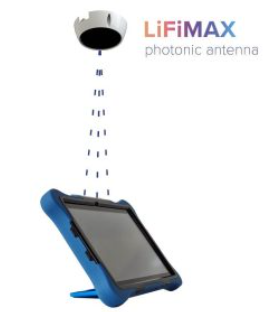
\includegraphics[width=40mm]{LiFiMAX.png}
    \caption{Li-FiMAX}
\end{figure}


\subsubsection*{MyLiFi lamp}

La làmpada MyLiFi és un llum d'escriptori amb una connectivitat LiFi segura, ràpida (23 Mb/s-) i sense ones de ràdio.

Les aplicacions mòbils i basades en web proporcionen control sobre la brillantor i la temperatura del color que van des del blanc càlid (2200K) fins a la llum del dia (6500K), permetent als usuaris crear el seu ambient preferit.


\begin{figure}[h!]
    \centering
    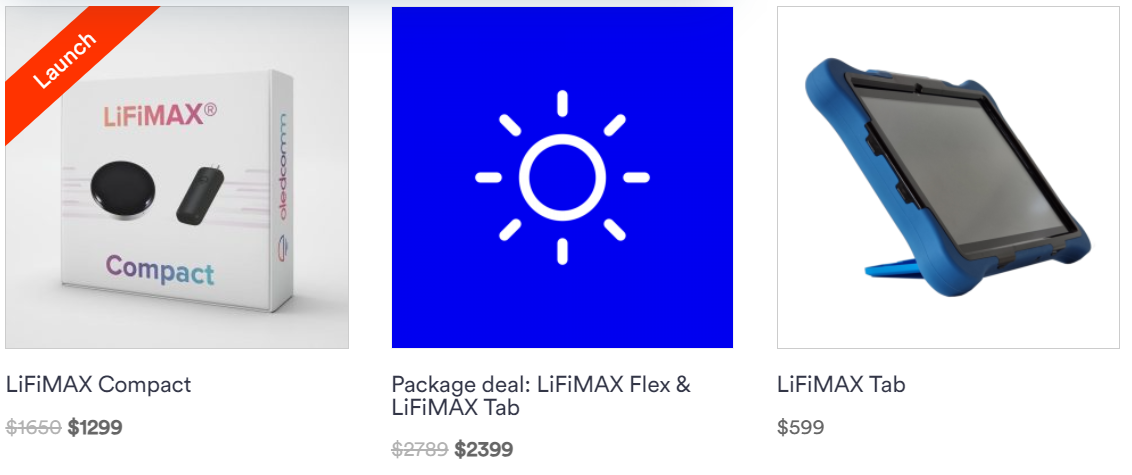
\includegraphics[width=80mm]{producteslifi.png}
    \caption{Altres productes Li-Fi i els seus preus}
\end{figure}